\section{Theorie}
\subsection{Newtonsche und Lagrange'sche Mechanik}
In folgenden soll die Herleitung der Bewegungsgleichung des Doppelpendels mit Hilfe des Lagrange-Formalismus der klassischen Mechanik beschrieben werden. \\
Die zu lösende Bewegungsgleichung eines Massepunkts ergibt sich nach Newton bekanntlich zu \begin{equation}
\vv{\ddot{x}}=\frac{1}{m}\sum \vv{F},
\end{equation} 
wobei $ \sum \vv{F} $ die Summe aller am Massepunkt angreifenden Kräfte, $\vv{x} $ die Ortskoordinate und $ m $ die Masse des betrachteten Massepunkts ist.
In der Praxis, so auch beim Doppelpendel, stellt es sich als äußerst schwierig dar, alle am Massepunkt wirkenden Kräfte zu identifizieren sowie mathematisch zu beschreiben. Als eine Art Verallgemeinerung der Newton'schen Mechanik lässt sich aus ihr der sogenannte Lagrange-Formalismus herleiten. Hier sind die gesuchten Funktionen die Lösungen der Lagrange-Gleichungen
\begin{equation}
\frac{d}{dt}\frac{\partial L}{\partial\dot{x_i}}-\frac{\partial L}{x_i} = 0
\end{equation}
mit der Lagrangefunktion  $ L=E_{kin} - V $ . Hierbei sind $E_{kin}$ die kinetische Energie und V das auf den Massepunkt wirkende Potential. Ein weiterer Vorteil dieses Formalismus besteht darin, dass die Langrangegleichungen unter Koordinatentransformationen invariant bleiben, es gilt also:
\begin{equation}
\frac{d}{dt}\frac{\partial L}{\partial\dot{q_i}}-\frac{\partial L}{q_i} = 0
\label{lagrangegl}
\end{equation}
Hier seien $q_i$ die sogenannten verallgemeinerten Koordinaten, die so gewählt werden, dass alle geometrischen Einschränkungen, denen das mechanische System unterworfen ist (sog. Zwangsbedingungen) berücksichtigt werden. Dies geschehe in dem Sinne, dass die verallgemeinerten Koordinaten für beliebige Werte nur unter den Zwangsbedingungen erlaubte Zustände liefern. Für jeden Freiheitsgrad muss nun eine Lagrangegleichung aufgestellt werden.
\subsection{Das Doppelpendel}
\begin{figure}
	\centering
	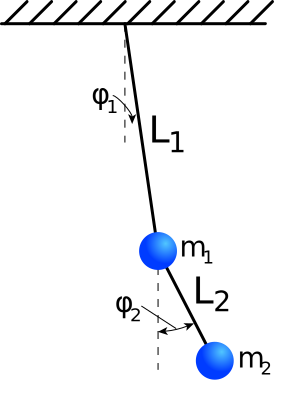
\includegraphics[width=.3\textwidth]{images/double-pendulum.png}
	\caption{Schematische Skizze eines Doppelpendels}
	\label{wiki:double-pendulum}
\end{figure}
Im Ursprungspunkt des Koordinatensystems wird ein Pendel, bestehend aus einem Stab mit fester Länge $l_1$ und einer Masse m an dessen Ende, befestigt. Das Pendel soll sich nur in der x-z Ebene bewegen können. Am Massenpunkt befindet sich nun ein zweites Pendel mit Stab der Länge $l_2$, welches sich ebenso nur in der x-z-Ebene bewegen soll. \\Es soll nun stets der Index 1 für Größen des oberen Pendels (inklusive der oberen Masse) und der Index 2 für alle Größen des unteren Pendels verwendet werden. \\
Der erste Schritt besteht nun darin, eine Beschreibung der Ortsvektoren der beiden Massenpunkte zu finden, die alle Zwangsbedingungen berücksichtigt. 
Derartige verallgemeinerte Koordinaten sind offenbar gegeben durch $ \varphi_1 $ und $ \varphi_2 $, welche die relativen Winkel der Stäbe $l_1 $ und $l_2$ zur Senkrechten (z-Achse) darstellen. Daraus folgt für $ \vv{x_1} $
\begin{equation}
\vv{x_1}= l_1\cdot\begin{pmatrix}
\sin \varphi_1 \\ -\cos \varphi_1
\end{pmatrix}
\end{equation}
Für den Vektor $\vv{x_2}$ folgt aus einfachen trigonometrischen Überlegungen:
\begin{equation}
\vv{x_2}= \vv{x_1} + l_2 \cdot \begin{pmatrix}
\sin \varphi_2 \\ -\cos \varphi_2
\end{pmatrix}
= \begin{pmatrix}
l_1 \cdot \sin \varphi_1 + l_2 \cdot \sin \varphi_2 \\ - l_1 \cdot \cos \varphi_1 - l_2 \cdot \cos \varphi_2
\end{pmatrix}
\end{equation}
Zur Bestimmung von $E_{kin,i} = \frac{m_i}{2} \cdot  \dot{\vv{x_i}}^2$  müssen noch die Ableitungen der Ortsvektoren gebildet werden:
\begin{equation}
\dot{\vv{x_1}} = l_1 \cdot \dot{\varphi_1} \cdot \begin{pmatrix}
\cos \varphi_1 \\ \sin \varphi_1
\end{pmatrix}
\end{equation}
und:
\begin{equation}
\dot{\vv{x_2}} = \dot{\vv{x_1}} + l_2 \cdot  \dot{\varphi_2} \cdot \begin{pmatrix}
\cos \varphi_2 \\ \sin \varphi_2
\end{pmatrix} 
\end{equation}
Für die kinetische Energie ergibt sich:
\begin{equation}
E_{kin} = E_{kin,1} + E_{kin,2} = \frac{m_1}{2} \cdot  l_1^2 \cdot  \dot{\varphi_1}^2 +
\frac{m_2}{2} \cdot (l_1^2 \cdot \dot{\varphi_1}^2 + l_2^2 \cdot \dot{\varphi_2}^2 + 2 \cdot l_1 \cdot l_2 \cdot \dot{\varphi_1} \cdot \dot{\varphi_2} \cdot \cos (\varphi_1 - \varphi_2))
\end{equation}
Das auf das Doppelpendel wirkende Potential $ V_i = m_i \cdot g \cdot h_i $ ist:
\begin{equation}
V = V_1 + V_2 = m_1 \cdot g \cdot (-l_1 \cdot \cos \varphi_1) + m_2 \cdot g \cdot (-l_1 \cdot \cos \varphi_1 - l_2 \cdot \cos \varphi_2)
\end{equation}
Das Aufstellen der Lagrange-Gleichung erfolgt nun in mehreren Schritten.\\ Zuerst für $ \varphi_1$ :
\begin{equation}
\frac{\partial (E_{kin} - V)}{\partial\dot{\varphi_1}} = (m_1 + m_2) \cdot l_1^2 \cdot \dot{\varphi_1} + m_2 \cdot (l_1 \cdot l_2 \cdot \dot{\varphi_2} \cdot \cos (\varphi_1 - \varphi_2)) 
\end{equation}
\begin{equation}
\frac{\partial (E_{kin} - V)}{\partial \varphi_1} = -m_2 l_1 l_2 \dot{\varphi_1} \dot{\varphi_2} \sin (\varphi_1 - \varphi_2) - (m_1 + m_2) g l_1 \sin \varphi_1
\end{equation}
und nun für $ \varphi_2 $ :

\begin{equation}
\frac{\partial (E_{kin} - V)}{\partial \dot{\varphi_2}} = m_2 l_2^2 \dot{\varphi_2} + m_2 l_1 l_2 \dot{\varphi_1} \cos (\varphi_1 - \varphi_2)
\end{equation}

\begin{equation}
\frac{\partial (E_{kin} - V)}{\partial \varphi_2} = m_2 l_1 l_2 \dot{\varphi_1} \dot{\varphi_2} \sin (\varphi_1 - \varphi_2) - m_2 g l_2 \sin \varphi_2
\end{equation}

Setzt man diese Terme in \eqref{lagrangegl} ein, erhält man die Bewegungsgleichungen des Systems:
\begin{equation}
\begin{split}
\frac{d}{dt}\frac{\partial L}{\partial\dot{\varphi_1}}-\frac{\partial L}{\varphi_1} = (m_1 + m_2) l_1^2\ddot{\varphi_1} + m_2 l_1 l_2 ( \ddot{\varphi_2} \cos (\varphi_1 - \varphi_2)+\\ + \dot{\varphi_2}^2 \sin (\varphi_1 - \varphi_2)) + (m_1 + m_2) g l_1 \sin \varphi_1 = 0
\end{split}
\end{equation}

\begin{equation}
\frac{d}{dt}\frac{\partial L}{\partial\dot{\varphi_2}}-\frac{\partial L}{\varphi_2} = m_2 l_2^2 \ddot{\varphi_2} + m_2 l_1 l_2 (\ddot{\varphi_1} \cos (\varphi_1 - \varphi_2) - \dot{\varphi_1}^2 \sin (\varphi_1 - \varphi_2)) + m_2 g l_2 \sin \varphi_2 = 0
\end{equation} 
Diese können noch vereinfacht werden durch eine Division durch $l_1$ bzw. $l_2$: 
\begin{equation}
\begin{split}
(m_1 + m_2) l_1\ddot{\varphi_1} + m_2 l_2 \ddot{\varphi_2} \cos (\varphi_1 - \varphi_2) + m_2 l_2 \dot{\varphi_2}^2 \sin (\varphi_1 - \varphi_2) +\\+ (m_1 + m_2) g \ sin \varphi_1 = 0
\end{split}
\label{equ:1}
\end{equation}
\begin{equation}
m_2 l_2 \ddot{\varphi_2} + m_2 l_1 (\ddot{\varphi_1} \cos (\varphi_1 - \varphi_2) - \dot{\varphi_1}^2 \sin (\varphi_1 - \varphi_2)) + m_2 g \sin \varphi_2 = 0
\label{equ:2}
\end{equation}

\subsection{Simulation des Doppelpendels}
Um die Gleichungen mittels eines Standardverfahrens numerisch lösen zu können, muss das Gleichungssystem (\ref{equ:1} und \ref{equ:2}) auf die Form $ \dot{Y} = f(Y) $ gebracht werden. Zunächst werden die obigen Gleichungen nach $ \ddot{\varphi_1} $ und $ \ddot{\varphi_2} $ aufgelöst. Es ergibt sich unter Beachtung der folgenden abkürzenden Notation: 
$ (m_1 + m_2) =: M; \varphi_1 - \varphi_2 =: \Delta \varphi $
\begin{equation}
\ddot{\varphi_1} = \frac{-m_2 l_2 \dot{\varphi_2}^{2} \sin{\Delta \varphi} - g M \sin{\varphi_1} - m_2 l_1 \dot{\varphi_1}^{2} \sin{\Delta \varphi} \cos{\Delta \varphi} + g m_2 \sin{\phi_2}\cos{\Delta  \varphi}}{M l_1 - m_2 l_1 \cos^{2}{\Delta \varphi}}
\end{equation}
und
\begin{equation} 
\ddot{\varphi_2} = \frac{-m_2 l_2 \dot{\varphi_2}^{2} \sin{\Delta \varphi} \cos{\Delta \varphi} - g M \sin{\varphi_1} \cos{\Delta \varphi} - M l_1 \dot{\varphi_1}^{2} \sin{\Delta \varphi} + g M \sin{\varphi_2}}{m_2 l_2 \cos^{2}{\Delta \varphi} - M l_2}
\end{equation}

Dieses Differenzialgleichungssystem erster Ordnung kann nun mit Hilfe elementarer Algorithmen gelöst werden. Hier wurde das expliztite Euler-Verfahren verwendet (\cite{eul}). Es wurde also ein Vektor $\vec{Y} = \vec{\varphi} = (
\varphi_1, \dot{\varphi_1}, \varphi_2 , \dot{\varphi_2})^{T} $
 definiert, für den sich ergibt: 
\begin{equation}
\dot{\vec{\varphi}} = (\dot{\varphi_1}, \ddot{\varphi_1}, \dot{\varphi_2}, \ddot{\varphi_2})^{T},
\end{equation}
wobei für $ \ddot{\varphi_1} $ und $ \ddot{\varphi_2} $ obige Gleichungen eingesetzt werden. 
Dann wird eine schrittweise Iteration durchgeführt, der Quelltext für das verwendete Python-Skript findet sich im Anhang. 

\subsection{Energieverlust des Systems}
Bei dem hier behandelten Doppelpendel treten im Wesentlichen Luftreibung und Reibung in der Lagerung der zueinander beweglichen Bauteile, also den Kugellagern, auf. Darüber hinaus tritt weiterer Energieverlust auf, indem die Aufhängung des Pendels vom Pendel selbst zu Schwingungen angeregt wird und so ein Energieübertrag stattfindet. 

\subsubsection{Luftreibung}
Für die Luftreibungskraft, die auf einen laminar umströmten Gegenstand wirkt, gilt die in guter Näherung gültige Formel
\begin{equation}
F_R = v^2 \cdot \frac{\rho}{2} \cdot A_S \cdot c_W,
\label{luftreibung}
\end{equation}
wobei $ F_R $ die Luftreibungskraft, $ v $ die Geschwindigkeit der umströmenden Luft, $ \rho $ deren Dichte, $ A_S $ die Fläche der Projektion des Gegenstands in Stömungsrichtung und $ c_W $ ein von der Form des Gegenstands bestimmter, dimensionsloser Koeffizient ist \cite{win}. 


\subsubsection{Reibung in den Kugellagern}
Für die Reibung in den Kugellagern kann das Modell der Rollreibung verwendet werden. Demnach ergibt sich für die Reibungskraft $ F_R $:
\begin{equation}
F_R = c_R \cdot F_N,
\end{equation} 
wobei $ c_R $ ein die verwendeten Materialien und deren Form charakterisierender Parameter ist und $ F_N $ der Betrag der Normalkraft, also die senkrecht zur Rollrichtung wirkende Kraft \cite{rol}. 

\subsubsection{Energieübertrag auf die Aufhängung}

Die Betrachtung dieser Art von Energieverlust ist schwierig. Er könnte mit dem Modell zweier gekoppelter schwingfähiger Systeme, bei dem das zweite eine große Dämpfung aufweist, angenähert werden. Allerdings müsste hierfür wieder der Lagrange-Formalismus herangezogen werden, wobei zusätzlich noch Reibungsterme berücksichtigt werden müssten. 

\subsection{Chaotisches Verhalten}
\subsubsection{Stabilität}
Die zeitliche Entwicklung vieler Systeme in der Mechanik kann durch lineare Differentialgleichungen beschrieben werden. Bei bekannten Anfangswerten können diese Gleichungen analytisch oder numerisch gelöst werden und damit die zeitliche Entwicklung des Systems komplett vorhergesagt werden, d.h. für exakte Anfangswerte gibt es exakte Vorhersagen für die zukünftige Entwicklung des Systems. Systeme dieser Art nennt man \textbf{streng deterministisch}. Wenn kleine Änderungen der Anfangswerte auch nur kleine Änderungen der zeitlichen Entwicklung nach sich ziehen, was mit Hilfe der Störungsrechnung bestimmt werden kann, nennt man die Lösung der Bewegungsgleichung \textbf{stabil}.
Bei anderen Systemen treten nichtlineare Differentialgleichungen als Bewegungsgleichungen auf. Bei diesen Systemen kommt es vor, dass kleine Änderungen der Anfangsbedingungen große Änderungen in der zeitlichen Entwicklung bewirken. Solche Lösungen nennt man  \textbf{instabil}, die Systeme bezeichnet man als \textbf{chaotisch}. Dies macht z.B. die Vorhersage von Vorgängen in der Natur sehr schwierig, da die Anfangsbedingungen schon allein aufgrund der Messungenauigkeit und der Menge an Informationen nicht genau bestimmt werden können. Trotzdem lassen sich im Rahmen der Chaosforschung einige interessante Aussagen über solche Systeme treffen, z.B. kann ein Maß für die Stabilität einer Lösung definiert werden und damit Vorhersagen getroffen werden.
\\

Ein sehr anschauliches Beispiel aus der Natur ist das Ringsystem des Saturn. Das Ringsystem hat einige gut sichtbare Lücken (Abbildung \ref{foto-saturn}), in denen sich keine der Staub- und Felsteilchen, aus denen die Ringe bestehen, befinden. Diese Lücken sind die Bereiche, in denen die Bewegungsgleichung eines Teilchens im Gravitationspotential des Saturn und seiner Monde keine stabile Lösung hat, sodass eine Umlaufbahn in diesen Bereichen nicht auf längere Zeit gehalten werden kann.
\\
\begin{figure}
\includegraphics[width=1.0\textwidth]{images/saturn.jpg}
\caption{Die Ringe des Saturn, aufgenommen von der Cassini-Sonde}
\label{foto-saturn}
\end{figure}

\subsubsection{Phasenraumkurven und Attraktoren}
Der Phasenraum eines Systems ist der Raum, dessen Koordinaten die Zustandsgrößen des Systems sind. (z.B. $x, \dot{x}$) Eine Kurve $X(t) = (x(t), \dot{x}(t))^T$ im Phasenraum heißt \textbf{Trajektorie} und beschreibt die zeitliche Entwicklung des Systems. Zeitlich konstante Punkte im Phasenraum, an denen die Geschwindigkeit des Massepunkts $\dot{X}(t) = 0$  ist, nennt man \textbf{Fixpunkte}. Kurven im Phasenraum können sich nur in Fixpunkten schneiden, da die zeitliche Entwicklung des Systems eindeutig durch die Anfangsbedingungen vorgegeben ist. Da in Fixpunkten mehrere (im Allgemeinen sogar unendlich viele) Trajektorien zusammenlaufen können, nennt man solche Fixpunkte auch \textbf{Attraktoren}. In nichtlinearen Systemen können Attraktoren auch andere Formen (z.B. Flächen oder Kurven) annehmen, sind dann aber keine Fixpunkte mehr.
\\
Phasenraumkurven sind ein praktisches Mittel, um das Verhalten von (chaotischen) Systemen zu zeigen, wie man in den folgenden Beispielen sehen kann.\footnote{\cite{troeder} Seite 386 ff.}

\begin{figure}
\includegraphics[width=1.0\textwidth]{images/phasenraum1.png}
\caption{Phasenraumkurven von: \\a) ungedämpfter harmonischer Oszillator \\b) gedämpfter harmonischer Oszillator \\c) harmonischer Oszillator mit negativer Dämpfung \\d) nichtlinearer angeregter Oszillator im chaotischen Bereich \\Herleitung siehe \cite{troeder} Seite 388}
\end{figure}

\begin{figure}
\includegraphics[width=1.0\textwidth]{images/phasenraum2.png}
\caption{Phasenraumkurven eines ungedämpften Fadenpendels. Der Punkt A ist Attraktor für alle Winkel $|\phi|<\pi$. Die rote Kurve stellt eine 'Grenzkurve' zwischen stabilen und instabilen Lösungen dar. Die Punkte B ($|\phi|=180^{\circ}, \dot{\phi}=0$) sind instabile Fixpunkte, eine minimale Änderung des Winkels wird eine stabile Pendelbewegung erzeugen, eine minimale Änderung der Winkelgeschwindigkeit wird eine Rotationsbewegung erzeugen, bei der der Winkel unbegrenzt ansteigt. \\
Herleitung siehe \cite{troeder} Seite 389}
\label{pic:pendel_einfach}
\end{figure}
